\documentclass[a4paper]{article}
  \usepackage{lipsum}
  \usepackage[margin=1in,left=1.5in,includefoot]{geometry}
  \usepackage{graphicx}
  \usepackage{graphicx}
\begin{document}
  \begin{titlepage}
  \begin{center}
  \line(1,0){300}\\
  [.25in]
  \huge{\bfseries Image Processing}\\
  [2mm]
  \line(1,0){200}\\
  [1.5cm]
  \textsc{\LARGE bangabandhu sheikh mujibur rahman science and technology university}\\
  [.75cm]
  \textsc{\Large latex first project}\\
  [10cm]
  \end{center}
  
  \begin{flushright}
  \textsc{\huge masud mia}\\
  A General Latex User\\
  18ICTCSE044\\
  january,2020
  \end{flushright}
  \end{titlepage}
  
 %front matter stuff
 \pagenumbering{roman}
 \section*{Summary}
 images using digital computers. Its use has been increasing exponentially in the last decades. Its applications range from medicine to entertainment, passing by geological processing and remote sensing. Multimedia systems, one of the pillars of the modern information society, rely heavily on digital image processing.
The discipline of digital image processing is a vast one, encompassing digital signal processing techniques as well as techniques that are specific to images. An image can be regarded as a function f (x, y) of two continuous variables x and y. To be processed digitally, it has to be sampled and transformed into a matrix of numbers. Since a computer represents the numbers using finite precision, these numbers have to be quantized to be represented digitally. Digital image processing consists of the manipulation of those finite precision numbers. The processing of digital images can be divided into several classes: image enhancement, image restoration, image analysis, and image compression. In image enhancement, an image is manipulated, mostly by heuristic techniques, so that a human viewer can extract useful information from it. Image restoration techniques aim at processing corrupted images from which there is a statistical or mathematical description of the degradation so that it can be reverted. Image analysis techniques permit that an image be processed so that information can be automatically extracted from it. Examples of image analysis are image segmentation, edge extraction, and texture and motion analysis. An important characteristic of images is the huge amount of information required to represent them. Even a gray-scale image of moderate resolution, say  Therefore, to be practical to store and transmit digital images, one needs to perform some sort of image compression, whereby the redundancy of the images is exploited for reducing the number of bits needed in their representation.

In what follows, we provide a brief description of digital image processing techniques. Section 4.1 deals with image sampling, and Section 4.2 describes image quantization. In Section 4.3, some image enhancement techniques are given. Section 4.4 analyzes image restoration. Image compression, or coding, is presented in Section 4.5. Finally, Section 4.6 introduces the main issues involved in image analysis.
\begin{figure}[h]
\centering

\includegraphics{bb}
\end{figure}

 
 \cleardoublepage
  
  %table of contents
  \tableofcontents
  \thispagestyle{empty}
  \cleardoublepage
  
  %main body stuff
  \pagenumbering{arabic}
  \setcounter{page}{1}  
  
  \section{Image sharpening and restoration
}
  Image sharpening and restoration refers here to process images that have been captured from the modern camera to make them a better image or to manipulate those images in way to achieve desired result. It refers to do what Photoshop usually does.

This includes Zooming, blurring , sharpening , gray scale to color conversion, detecting edges and vice versa , Image retrieval and Image recognition. The common examples are:
\begin{figure}[h]
\centering
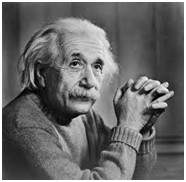
\includegraphics[width=5in,height=4in]{ms}
\caption{Einstein}
\end{figure}
 \section{Medical field}
 The common applications of DIP in the field of medical is
  \begin{itemize}
    \item Gamma ray imaging
  \item PET scan
  \item X Ray Imaging
  \item Medical CT
  \item UV imaging
  \end{itemize}
  \newpage
 \section{UV imaging}
 In the field of remote sensing , the area of the earth is scanned by a satellite or from a very high ground and then it is analyzed to obtain information about it. One particular application of digital image processing in the field of remote sensing is to detect infrastructure damages caused by an earthquake.

As it takes longer time to grasp damage, even if serious damages are focused on. Since the area effected by the earthquake is sometimes so wide , that it not possible to examine it with human eye in order to estimate damages. Even if it is , then it is very hectic and time consuming procedure. So a solution to this is found in digital image processing. An image of the effected area is captured from the above ground and then it is analyzed to detect the various types of damage done by the earthquake.
\begin{figure}[h]
\centering
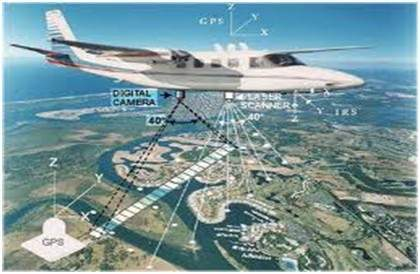
\includegraphics{sm}
\end{figure}
The key steps include in the analysis are
\begin{itemize}
\item The extraction of edges
\item Analysis and enhancement of various types of edges
\end{itemize}
\newpage
 
  \section{Transmission and encoding}
The very first image that has been transmitted over the wire was from London to New York via a submarine cable. The picture that was sent is shown below.
\begin{figure}[h]
\centering
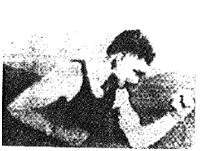
\includegraphics{pp}
\end{figure}
The picture that was sent took three hours to reach from one place to another.

Now just imagine , that today we are able to see live video feed , or live cctv footage from one continent to another with just a delay of seconds. It means that a lot of work has been done in this field too. This field doesnot only focus on transmission , but also on encoding. Many different formats have been developed for high or low bandwith to encode photos and then stream it over the internet or e.t.c.
 \section{Machine/Robot vision}
 Apart form the many challenges that a robot face today , one of the biggest challenge still is to increase the vision of the robot. Make robot able to see things , identify them , identify the hurdles e.t.c. Much work has been contributed by this field and a complete other field of computer vision has been introduced to work on it.
  
  \section{Hurdle detection}
  Hurdle detection is one of the common task that has been done through image processing, by identifying different type of objects in the image and then calculating the distance between robot and hurdles.
  \begin{figure}[h]
  \centering
  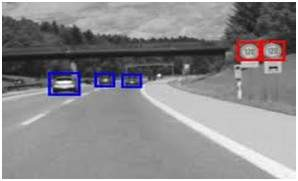
\includegraphics{mm}
  \end{figure}
  
  \section{Line follower robot}
  Most of the robots today work by following the line and thus are called line follower robots. This help a robot to move on its path and perform some tasks. This has also been achieved through image processing.

\begin{figure}[h]
\centering

\includegraphics{op}
\end{figure}
 \section{Color processing}
 Color processing includes processing of colored images and different color spaces that are used. For example RGB color model , YCbCr, HSV. It also involves studying transmission , storage , and encoding of these color images.
  \section{Pattern recognition}
   Pattern recognition involves study from image processing and from various other fields that includes machine learning ( a branch of artificial intelligence). In pattern recognition , image processing is used for identifying the objects in an images and then machine learning is used to train the system for the change in pattern. Pattern recognition is used in computer aided diagnosis , recognition of handwriting , recognition of images e.t.c
\section{Video processing}
  A video is nothing but just the very fast movement of pictures. The quality of the video depends on the number of frames/pictures per minute and the quality of each frame being used. Video processing involves noise reduction , detail enhancement , motion detection , frame rate conversion , aspect ratio conversion , color space conversion e.t.c.
\newpage 
 \section{How human eye works?
}
   Before we discuss , the image formation on analog and digital cameras , we have to first discuss the image formation on human eye. Because the basic principle that is followed by the cameras has been taken from the way , the human eye works.

When light falls upon the particular object , it is reflected back after striking through the object. The rays of light when passed through the lens of eye , form a particular angle , and the image is formed on the retina which is the back side of the wall. The image that is formed is inverted. This image is then interpreted by the brain and that makes us able to understand things. Due to angle formation , we are able to perceive the height and depth of the object we are seeing. This has been more explained in the tutorial of perspective transformation.
\begin{figure}[h]
\centering
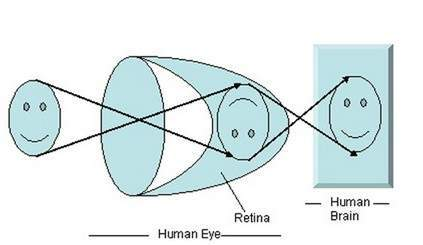
\includegraphics{dd}
\end{figure}
As you can see in the above figure, that when sun light falls on the object (in this case the object is a face), it is reflected back and different rays form different angle when they are passed through the lens and an invert image of the object has been formed on the back wall. The last portion of the figure denotes that the object has been interpreted by the brain and re-inverted.

Now lets take our discussion back to the image formation on analog and digital cameras
\newpage

  \section{Image formation on analog cameras}
   \begin{figure}[h]
   \centering
   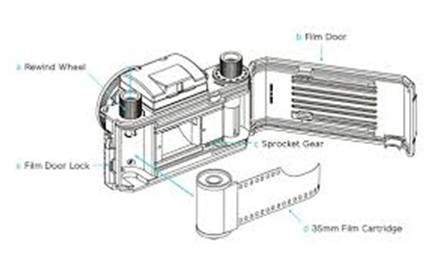
\includegraphics{aa}
   \end{figure}
   In analog cameras , the image formation is due to the chemical reaction that takes place on the strip that is used for image formation.

A 35mm strip is used in analog camera. It is denoted in the figure by 35mm film cartridge. This strip is coated with silver halide ( a chemical substance)
A 35mm strip is used in analog camera. It is denoted in the figure by 35mm film cartridge. This strip is coated with silver halide ( a chemical substance).

Light is nothing but just the small particles known as photon particles.So when these photon particles are passed through the camera, it reacts with the silver halide particles on the strip and it results in the silver which is the negative of the image.

In order to understand it better , have a look at this equation.

Photons (light particles) + silver halide ? silver ? image negative
This is just the basics, although image formation involves many other concepts regarding the passing of light inside , and the concepts of shutter and shutter speed and aperture and its opening but for now we will move on to the next part. Although most of these concepts have been discussed in our tutorial of shutter and aperture.

This is just the basics, although image formation involves many other concepts regarding the passing of light inside , and the concepts of shutter and shutter speed and aperture and its opening but for now we will move on to the next part. Although most of these concepts have been discussed in our tutorial of shutter and aperture.

\newpage
  \section{Image formation on digital cameras
}
  Image formation on digital cameras
In the digital cameras , the image formation is not due to the chemical reaction that take place , rather it is a bit more complex then this. In the digital camera , a CCD array of sensors is used for the image formation.

\section{Image formation through CCD array}
  \begin{figure}[h]
  \centering
  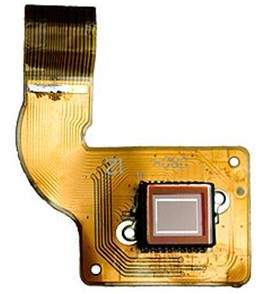
\includegraphics{uu}
  \end{figure}
  CCD stands for charge-coupled device. It is an image sensor, and like other sensors it senses the values and converts them into an electric signal. In case of CCD it senses the image and convert it into electric signal e.t.c.

This CCD is actually in the shape of array or a rectangular grid. It is like a matrix with each cell in the matrix contains a censor that senses the intensity of photon.

\begin{figure}[h]
\centering
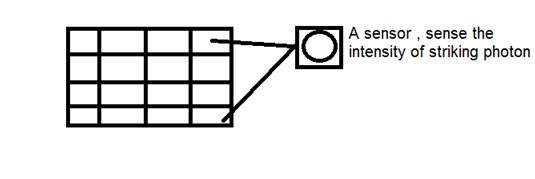
\includegraphics{tt}
\end{figure}
Like analog cameras , in the case of digital too , when light falls on the object , the light reflects back after striking the object and allowed to enter inside the camera.

Each sensor of the CCD array itself is an analog sensor. When photons of light strike on the chip , it is held as a small electrical charge in each photo sensor. The response of each sensor is directly equal to the amount of light or (photon) energy striked on the surface of the sensor.

Since we have already define an image as a two dimensional signal and due to the two dimensional formation of the CCD array , a complete image can be achieved from this CCD array.

It has limited number of sensors , and it means a limited detail can be captured by it. Also each sensor can have only one value against the each photon particle that strike on it.

So the number of photons striking(current) are counted and stored. In order to measure accurately these , external CMOS sensors are also attached with CCD array.

 \section{Storing image
}
The charges stored by the CCD array are converted to voltage one pixel at a time. With the help of additional circuits , this voltage is converted into a digital information and then it is stored.

Each company that manufactures digital camera, make their own CCD sensors. That include , Sony , Mistubishi , Nikon ,Samsung , Toshiba , FujiFilm , Canon e.t.c.

Apart from the other factors , the quality of the image captured also depends on the type and quality of the CCD array that has been used.
  \section{Camera Mechanism}
 \begin{figure}[h]
\centering
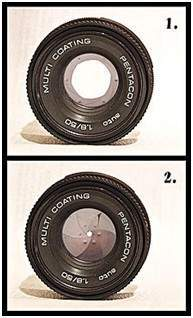
\includegraphics{ll}
\caption{aperture}
\end{figure} 
  \subsection{Aperture}
  Aperture is a small opening which allows the light to travel inside into camera. Here is the picture of aperture.
You will see some small blades like stuff inside the aperture. These blades create a octagonal shape that can be opened closed. And thus it make sense that, the more blades will open, the hole from which the light would have to pass would be bigger. The bigger the hole, the more light is allowed to enter.
\newpage
\section{Concept of Pixel
}
\subsection{Pixel}
Pixel is the smallest element of an image. Each pixel correspond to any one value. In an 8-bit gray scale image, the value of the pixel between 0 and 255. The value of a pixel at any point correspond to the intensity of the light photons striking at that point. Each pixel store a value proportional to the light intensity at that particular location.

\subsection{PEL}
A pixel is also known as PEL. You can have more understanding of the pixel from the pictures given below.
\newpage
\section{Calculation of total number of pixels}
We have define an image as a two dimensional signal or matrix. Then in that case the number of PEL would be equal to the number of rows multiply with number of columns.

This can be mathematically represented as below:

Total number of pixels = number of rows ( X ) number of columns

Or we can say that the number of (x,y) coordinate pairs make up the total number of pixels.

We will look in more detail in the tutorial of image types, that how do we calculate the pixels in a color image.
\section{Gray level}
The value of the pixel at any point denotes the intensity of image at that location, and that is also known as gray level.

We will see in more detail about the value of the pixels in the image storage and bits per pixel tutorial, but for now we will just look at the concept of only one pixel value.
\section{Shutter}
After the aperture, there comes the shutter. The light when allowed to pass from the aperture, falls directly on to the shutter. Shutter is actually a cover, a closed window, or can be thought of as a curtain. Remember when we talk about the CCD array sensor on which the image is formed. Well behind the shutter is the sensor. So shutter is the only thing that is between the image formation and the light, when it is passed from aperture.

As soon as the shutter is open, light falls on the image sensor, and the image is formed on the array.



\end{document}